\chapter{Introduction}
\label{chap:intro}

In present-day economic circumstances, businesses are presented with numerous challenges. Some of those challenges originate form the businesses themselves, like for example the strategic aim of growing and expanding into new markets, or the forging of customer and market awareness. Other challenges originate from the business and regulatory environment of the business in question. These environments force a business to be ever more competitive and to optimize for sustainability. To achieve this, industries no longer put the product itself at the core. Rather, they incorporate the product into a number of services, which reach from the lowest-level technical detail to the highest-level customer interaction and provide for optimal product utilization. In this sense, what a company tries to sell nowadays is not just the product itself, but a service through which the customer consumes the product, while being isolated from technical detail and unnecessary responsibility. Such complete solutions are denoted as \gls{PSS}.

While the incorporation of Product-Service Systems in an industry requires an initial effort and an evolution of the companies' cultures, it can lead to a more concise and efficient utilization of resources to the benefit of both the companies themselves and their customers. 

\section*{Importance of Integration}

After their implementation and market introduction, Product-Service Systems can bring numerous benefits to a company. Nevertheless, their implementation brings a number of challenges of communication, integration and complexity. To explain this, let us consider the parties involved in the development and production cycles of a \gls{PSS}. Both development and production involve a number of disciplines, each acquainted with its own modelling languages and tools. Each of these domain-specific languages furthermore is concerned only with those aspects of the overall systems, which are relevant for the discipline at hand. As a result, each involved party has only a limited excerpt of the entire \gls{PSS} at its disposal. In the worst case, this leads to contradictions in the design and implementation of the system. In the moderate case, it only incurs significant synchronization and management costs to the company. It is thus of crucial importance for the success of a PSS venture to establish a mechanism though which the models developed by different disciplines can be transformed to each other, or even to incorporate them all in a single model, representing the \gls{PSS} in its entirety.

\section*{PSS Integration Framework}

An approach to the integration of the disciplines involved in the development of a \gls{PSS} is researched jointly in the faculties of Informatics and Mechanical Engineering of the Technical University of Munich by C. M\"unzberg, D. Kammerl, K. Kernschmidt and T. Wolfenstetter. The approach is named \gls{PSSIF} and provides a methodology and semantics for bringing the business, computer science and mechanical engineering aspects of a \gls{PSS} together. In its core, the framework describes a common structure which is sufficiently expressive to incorporate the \gls{PSS} wide relevant features of each domain-specific aspect of the PSS. This structure is depicted in \figref{fig:canonic}.

\begin{figure}
\centering
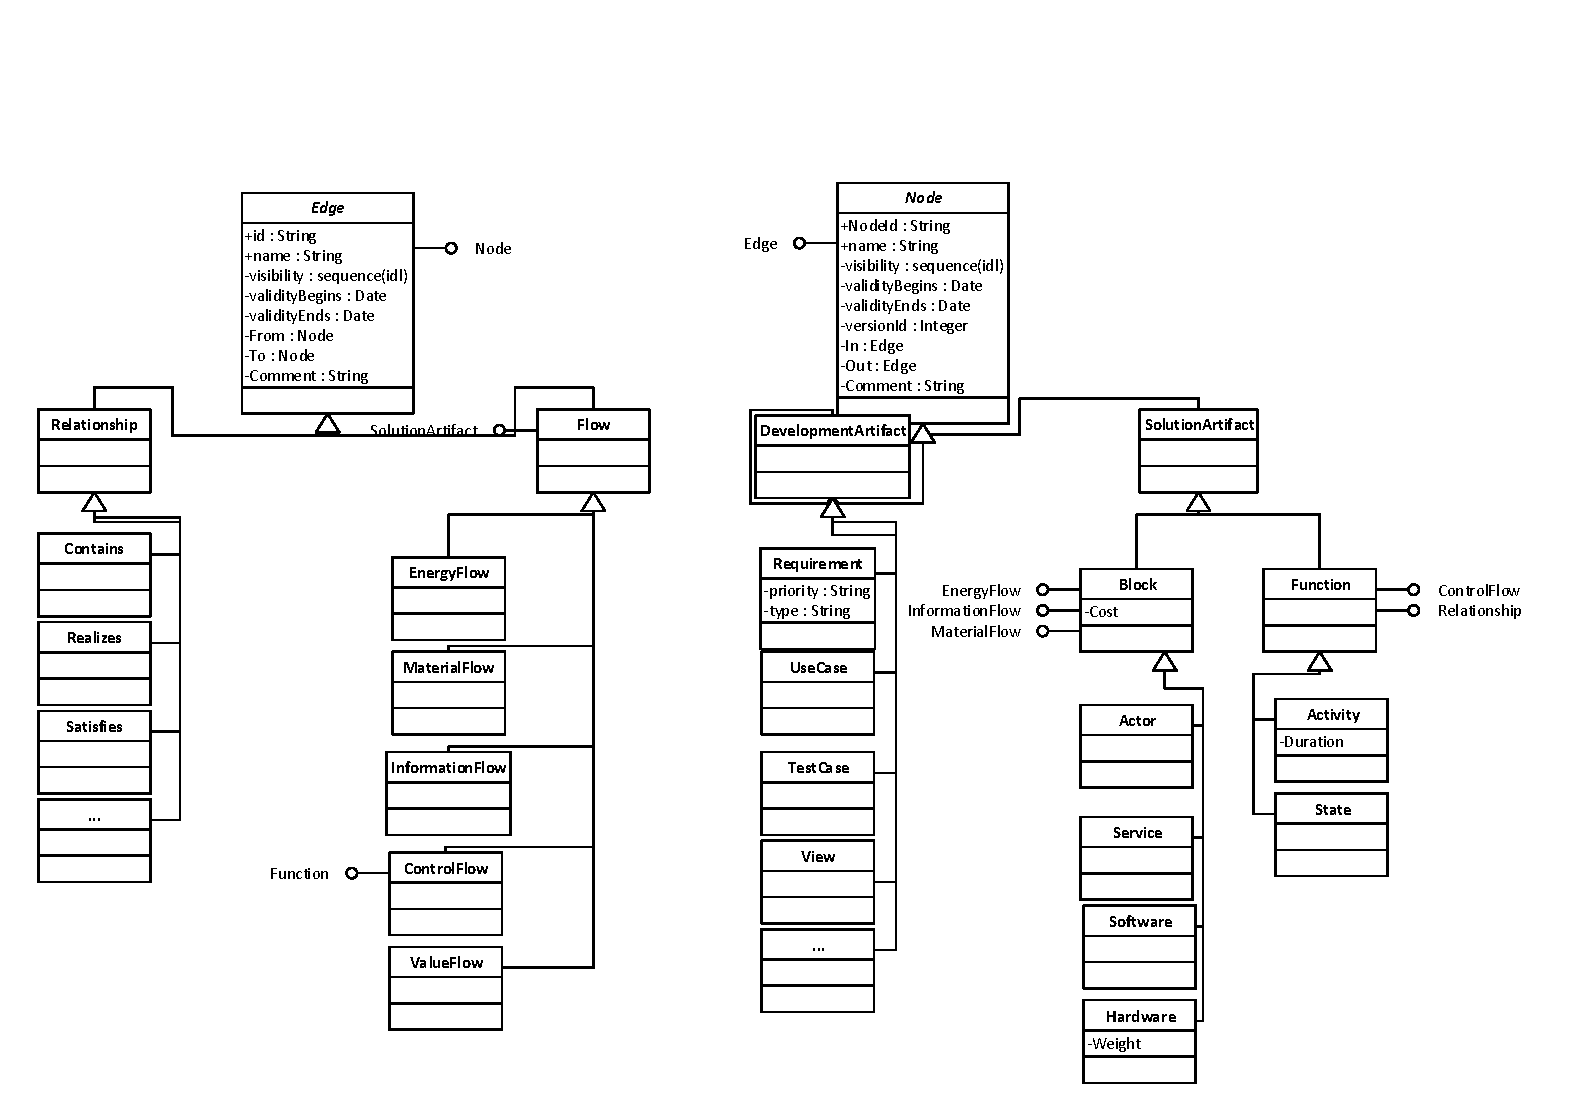
\includegraphics[width=\textwidth]{figures/PSSIF.pdf}
\caption{PSS-Integration Framework Common Structure}
\label{fig:canonic}
\end{figure}

The main goal of the \gls{PSSIF} is the usage of this structure for the integration of models of different disciplines. For this purpose, a key step is the ability to translate models from and to this common structure.

\section*{Scope of the Interdisciplinary Project}

In the context of the \gls{PSSIF}, the goal is to design and implement a \gls{poc} software utility which:

\begin{itemize}
\item follows the PSS-IF methodology and semantics,
\item can transform a model described in one relevant domain-specific language into another relevant domain-specific language,
\item considers the following domain-specific languages relevant:
	\begin{itemize}
	\item Event-driven Process Chain (EPC) Diagrams
	\item Business Process Modelling Notation (BPMN) Diagrams
	\item Flow-oriented Functional Modelling (FFM) Diagrams modelled using the BOOGGIE-Tool (Bringing Object-oriented Graph Grammars into Engineering)
	\item Systems Modelling Language for Mechatronics (SysML4Mechatronics) Diagrams and,
	\end{itemize}
\item should, at the time of its delivery, support at least two of the relevant domain-specific languages.
\end{itemize} 

\section*{Structure of this Documentation}
In \chapref{chap:approach} we discuss possible approaches to the conceptual structure of the \gls{poc} developed in this interdisciplinary project. \chapref{chap:impl} describes the implementation of the \gls{poc}. The results obtained from the \gls{poc} are described in \chapref{chap:results}. In {\chapref{chap:outlook} we furthermore provide a few ideas about possible future developments on the basis of the provided \gls{poc}.


